\documentclass[12pt]{article}
\usepackage[utf8]{inputenc}
\usepackage{graphicx}
\usepackage{subcaption}
\usepackage{forest}
\usepackage{amsmath}
\usepackage{cite}
\usepackage{hyperref}

\title{
  
\includegraphics[height=1.6cm]{pictures/SUSig_2color_Stree_StnfrdOnly_Left.png}
  \hspace{1.5cm}
  
\includegraphics[height=1.6cm]{pictures/logo-epfl-1024x576.png}
  \\[4mm]
  \large Real-Time Multimodal Performance Assessment for dVRK \\[3mm]
  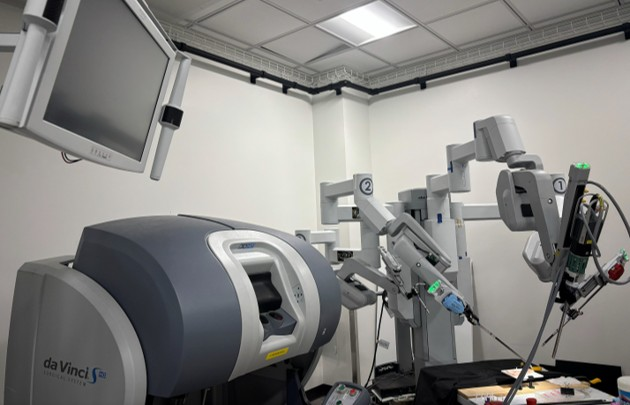
\includegraphics[width=0.7\textwidth]{pictures/dvrk.jpg}
}
\author{
  \normalsize
  Shujiro Shobayashi \\[2mm]
  \large
  Supervisors: \\
  Prof. Allison Okamura (Stanford University) \\
  Prof. Josephine Hughes (EPFL) \\[1mm]
  Mentors: \\
  Mary Kate Gale, Brian Vuong
}
\date{\today}

\begin{document}

\maketitle

\newpage

\begin{abstract}
Real-time performance feedback can accelerate skill acquisition during
robotic surgical training, but existing systems either compute
performance measures only after a task ends (post-hoc), or depend on a
human rater to trigger and score feedback during the trial. We present
a multimodal system that measures peg-transfer task performance live,
on a physical da Vinci Research Kit, with no human rater at any point
in the loop. The system fuses kinematic, visual, and force data through
an event-triggered pipeline: trial time and instrument path length are
tracked in real time, cylinder orientation is checked at placement via
HSV segmentation on a YOLOv8-detected cylinder, and contact force is
reported immediately after each trial. In addition, with the depth
camera, we collect a higher-accuracy, SAM2-based 3D localization
measure post-hoc, as extra validation data for the real-time measures.
We demonstrate the system on the physical robot, validating the
real-time measures against this higher-accuracy post-hoc reference, and
show that automated, real-time, on-robot performance measurement is
feasible for a structured surgical training task; laying the
groundwork for a closed-loop, difficulty-adaptive training system.
\end{abstract}

\newpage
\tableofcontents

\section{Introduction}

\subsection{Scope}

This thesis makes one deliberate scope decision: it scores performance on a
single, well-defined task, not global surgical skill. Task scoring reduces
the problem to metrics that are objective and computable in real time --
completion time, path length, angular displacement, object state. Surgical
skill is broader, harder to define, and harder to measure objectively. Task
scoring is also solvable within a six-month thesis; general skill assessment
is not. This choice, not a limitation discovered later, shapes every design
decision in the chapters that follow.

\subsection{Goal}

The goal is real-time assessment of task performance on the da Vinci
Research Kit (dVRK), delivered as feedback during the task rather than
through post-hoc review. The target task is peg transfer: the trainee moves
a cylinder between pegs on a task pad under stereo endoscopic vision.

The system scores each trial automatically and objectively, without a human
rater in the loop. Four measures form the score: completion time, path
length of the instrument tip, angular displacement of the grasped object,
and object state (stationary, held, or dropped). Automatic scoring removes
inter-rater variability and makes the score available while the trial is
still running, not after the trainee has left the console.

The long-term vision extends past a single scored trial: a closed-loop
system that adapts task difficulty to the trainee's demonstrated
performance, without an instructor setting parameters by hand. The
adaptive-task design in Section~\ref{sec:conclusion} outlines one path
toward that vision; this thesis builds the real-time measurement layer
that any such closed loop would depend on.

\subsection{Motivation}

\paragraph{Real-time feedback accelerates learning.} Trainees who see their
performance while still performing the task can correct technique
immediately, instead of waiting for a debrief after the console session
ends. Immediate, task-relevant feedback is established in the motor-skill
learning literature as more effective for skill acquisition than delayed,
post-session review~\cite{TODO_motor_learning}. A real-time score turns
every trial into a feedback opportunity, not just a data point for later
analysis.

\paragraph{Automated capture catches what human observers miss.} An
expert observer watching a live trial cannot track every event at once --
a brief arm collision, incidental contact with the environment, a subtle
wrist over-rotation. These events are easy to miss in real time and hard
to reconstruct afterward from memory or video alone. Sensor-driven capture
logs every such event with precision, producing a complete record that
does not depend on what the observer happened to notice.

\paragraph{Multimodal data can surface metrics that redefine proficiency.}
Completion time is the traditional proxy for skill, but it collapses a lot
of information into one number. Combining kinematic, visual, and force data
opens the door to metrics that time alone cannot express -- motion
smoothness, instrument path efficiency, grasp stability. These metrics may
distinguish expert from novice behavior more precisely than time does, and
could inform how surgical proficiency is measured beyond this task.

\subsection{Contribution}

Prior work establishes the two ends of this problem separately: offline
kinematic analysis scores skill accurately but after the fact, and
real-time feedback systems exist but depend on a human expert to trigger
them (see Chapter~\ref{sec:background} for the detailed comparison). This
thesis closes that gap for one task: a multimodal, automated system that
scores dVRK peg transfer live, on the physical robot, with no human rater
and no post-hoc processing step in the feedback loop.

\section{Background \& Related Work}

Test here
\section{System Design \& Task Setup}
\label{sec:system_design}

\subsection{Hardware}

Experiments were run on a da Vinci Research Kit (dVRK)~\cite{dvrk}. The
dVRK pairs a da Vinci S surgeon-side console with da Vinci Si
patient-side arms, instrumented with bipolar fenestrated forceps. Two
patient-side manipulators, PSM1 and PSM2, are available for control;
trials can use either arm alone or both together.

\subsection{Task}
\label{subsec:task}

The task is a cylinder-on-peg transfer task. The task board holds four
blue and four white cylinders at rest on four center pegs. Eight pegs
ring the outside of the board; each is embedded with an LED that lights
either blue or white to indicate the target cylinder and its destination
peg for the next move (Figure~\ref{fig:task_board}).

The board is instrumented with conductive paint, wired to detect cylinder
placement and removal directly: contact between a cylinder and a peg
closes a circuit specific to that peg. This gives a ground-truth signal
for cylinder state -- seated on a peg, or in transit -- independent of
the vision pipeline.

\begin{figure}[h]
\centering
% \includegraphics[width=0.6\textwidth]{figures/task_board.png}
\caption{Task board layout. Four center pegs hold the cylinders at rest.
Eight outer pegs illuminate blue or white via embedded LEDs to indicate
the target cylinder and destination for the next move.}
\label{fig:task_board}
\end{figure}

\subsection{Vision}
\label{subsec:vision}

Two camera streams feed the pipeline. The dVRK endoscopic camera provides
the stereo view used at the surgeon console. An Intel RealSense D405
depth camera, mounted next to the task board, provides a fixed external
RGB-D view of the workspace, independent of console head motion.
% TODO: auxiliary camera view -- extra pedal toggles a second view
% (top or side of task pad) during robot control, for added depth
% perception. Describe pedal mapping and where the view is displayed.

\subsection{Sensing}
\label{subsec:sensing}

Three further modalities complement the two camera streams. Kinematic
data -- joint positions, velocities, and tool-tip pose -- is read
directly from the patient-side manipulators (PSMs). Task start and end
events are detected by an Arduino-based trigger circuit, independent of
the vision and kinematic streams. Contact forces are measured by an ATI
force sensor mounted underneath the task pad, capturing forces
transmitted through the board as cylinders are placed and removed.

\section{Methods}
\label{sec:methods}

\subsection{Pipeline Overview}
\label{subsec:pipeline_overview}

The measures below come from one integrated pipeline, not independent
scripts. Lifting the cylinder off its center peg triggers the Arduino
board signal (Section~\ref{subsec:task}); this starts the GUI trial
clock and begins path-length accumulation. Placing the cylinder on its
target peg triggers the matching Arduino signal and stops the clock. At
that instant, HSV segmentation on the YOLOv8-detected~\cite{yolov8} cylinder estimates
its orientation and checks whether the correct face -- blue or white, as
indicated by the lit target peg (Section~\ref{subsec:task}) -- ended
face down. Once the trial ends, the GUI plots the total force applied to
the task pad during the trial: time on the x-axis, force in newtons on
the y-axis, read from the ATI sensor.

Table~\ref{tab:data_timing} summarizes every measure the pipeline
collects: its timing class, what triggers it, and how it reaches the
trainee.

\begin{table}[h]
\centering
\resizebox{\textwidth}{!}{%
\begin{tabular}{|p{5.2cm}|p{3.5cm}|p{5.6cm}|p{5.6cm}|}
\hline
\textbf{Data / Measure} & \textbf{Timing} & \textbf{Trigger} &
\textbf{Feedback} \\
\hline
Trial time &
Real-time &
Continuous, lift-to-placement &
Progress bar (GUI) \\[4pt]
\hline
Path length &
Real-time &
Continuous while clock runs &
Numeric running total \\[4pt]
\hline
Object detection (YOLOv8~\cite{yolov8}) &
Real-time, delayed &
Continuous, event-triggered at placement &
Backbone for orientation \& state below \\[4pt]
\hline
Cylinder orientation (HSV) &
Real-time, delayed &
Continuous, event-triggered at placement &
Binary indicator \\[4pt]
\hline
Object state (4 classes) &
Real-time &
Continuous &
Status indicator \\[4pt]
\hline
Contact force &
Real-time, delayed &
Continuous, after trial ends &
2D graph, time (x) vs.\ force in N (y) \\[4pt]
\hline
Additional camera &
Real-time &
Continuous, pedal-triggered &
Additional camera view \\[4pt]
\hline
3D localization (SAM2~\cite{sam2}) &
Post-hoc &
Offline processing &
Not shown to trainee; offline plot \\
\hline
\end{tabular}%
}
\caption{Data collected by the pipeline, its timing class, trigger, and
the feedback form it reaches the trainee in}
\label{tab:data_timing}
\end{table}

\subsection{Real-Time GUI \& Trial Clock}

The trial clock starts and stops from the Arduino cylinder-lift/placement
signal (Section~\ref{subsec:pipeline_overview}), not from pedal state.
Path length accrues on the GUI for the full duration the clock runs.
% TODO: code to be copied into code/ from external folder once path is
% provided.

\subsection{Object Detection}
% TODO: YOLOv8 detector, trained on 4 classes -- cylinders, inactive
% pegs, blue pegs, white pegs. Feeds the angular-displacement and
% object-state methods below.

\subsection{Path Length}
% TODO

\subsection{Angular Displacement}
\label{subsec:angular_displacement}

Cylinder orientation is estimated by HSV segmentation on the region
YOLOv8 detects as the cylinder.
% TODO: describe the HSV method itself -- color thresholds, how the
% orientation angle is derived from the segmented mask.

This estimate is computed at placement and feeds the
orientation-correctness check in Object State Detection below.

\subsection{Object State Detection}

At placement, the orientation estimate from
Section~\ref{subsec:angular_displacement} determines whether the
cylinder landed correctly: the lit target peg (Section~\ref{subsec:task})
specifies blue or white face down, and the trial is scored correct or
incorrect against that target.
% TODO: classifier over 4 cylinder states -- stationary, held, dropped,
% lost -- augmented with XGBoost. Cross-check against conductive-paint
% task board signal (subsec:task) and ground contact detection below.

\subsection{Ground Contact Detection}

Contact force from the ATI sensor is not streamed live during the trial.
Once the trial ends, the GUI displays it as a 2D graph -- time on the
x-axis, total force in newtons on the y-axis -- showing how much force
was applied to the task pad over the course of the trial.

\subsection{3D Localization (Post-Hoc)}

The pipeline includes a 3D localization method for the cylinder, tracking
its $(x, y, z)$ position from the RealSense D405 depth stream. An early
version of this method ran in real time, but tracking was unreliable.
% TODO: state the specific failure mode (noise / occlusion / drift / other)
To improve accuracy, the method was rebuilt on Segment Anything 2
(SAM2)~\cite{sam2} for cylinder segmentation. SAM2 produces an accurate
mask, but its per-frame runtime exceeds the trial's real-time budget.

This method therefore runs post-hoc, after the trial ends, not live
during it. Its role in this thesis is validation, not live measurement:
3D localization gives an accurate offline reference for cylinder
position, used to check the real-time measures -- path length and
angular displacement -- against ground truth. It is not one of the
real-time measures the system delivers during a trial
(Section~\ref{subsec:scope}).
\section{Results}
\label{sec:results}

The results below come from bench trials run by the author on the
physical dVRK, used to validate that the pipeline works as described
in Section~\ref{sec:methods}, not from a study with trainees; that
study is future work (Section~\ref{sec:conclusion}). Rather than
validating each measure in isolation, this chapter follows the same
logic as the pipeline itself (Section~\ref{subsec:pipeline_overview}):
the measures are merged into one system, so results are shown as what
one trial, run through the whole pipeline at once, actually produces,
with timing broken out on its own, since it calls for a direct,
quantitative check against the real-time claim this thesis makes.

\subsection{An Integrated Trial}
\label{subsec:results_integrated_trial}

% PLACEHOLDER: walk through one representative trial end to end, in
% the order the pipeline itself produces it (Section~\ref{subsec:pipeline_overview}):
% trial time and path length live in the GUI; rate of orientation
% change printed to the terminal; the upright/color-down check and
% object-state classification at placement; the force popup after the
% trial ends. The point is to show these together, as the trainee
% would actually see them from a single trial, not as separate
% one-off numbers.
% TODO: pick 1-3 representative trials (e.g. a clean success, a drop,
% a wrong-color placement) and report what every measure showed for
% each, ideally with a screenshot/photo of the GUI and force popup.

\subsection{Timing}
\label{subsec:results_timing}

This thesis claims the pipeline is real-time. This section checks
that claim directly, per module, against measured timing rather than
against the code's own assumptions about itself.

Trial time, path length, and rate of orientation change
(Section~\ref{subsec:kinematic_metrics}) update continuously while the
clock runs, driven by a background process that assumes a 200~Hz
internal clock (Section~\ref{subsec:gui_trial_clock}). The measured
update rate, both how often the GUI actually refreshes and how often
new PSM pose samples actually arrive, was [TODO] Hz.

The orientation check (Section~\ref{subsec:angular_displacement}) has
a built-in 0.5~s settle delay after the Arduino's ``Target hit''
signal, plus processing time, plus up to two further 0.5~s retries if
the cylinder is not found in the crop. Measured from that event to the
printed result, over [TODO] trials, the time was [TODO]~s on average
and [TODO]~s at the slowest.

The object-state classifier (Section~\ref{subsec:object_state}) runs
once per frame; its measured inference time, over [TODO] calls, was
[TODO]~ms on average and [TODO]~ms at the slowest.

The force popup (Section~\ref{subsec:ground_contact}) appears once a
trial ends; the measured time from trial end to the popup becoming
visible was [TODO]~s.

\section{Discussion}
\label{sec:discussion}

\subsection{Does This Close the Gap?}

Section~\ref{sec:background} lined up related work against three
requirements, automated, real-time, and on physical hardware, and
found that no prior approach met all three at once
(Table~\ref{tab:related_work}). This system computes trial time, path
length, and rate of orientation change directly from PSM kinematics,
checks cylinder orientation and object state directly from vision,
and reports contact force, all without a human rater, on the physical
dVRK, during the trial itself (Section~\ref{sec:methods}). The one
exception is 3D localization, which runs post-hoc, not live; but it
was never delivered as one of the real-time measures
(Section~\ref{subsec:localization}), it exists to validate the
others, so it is not itself a gap in that claim.
% TODO: revisit this once Results is complete, in case the timing
% numbers change this conclusion.

\subsection{What the Timing Means}
\label{subsec:discussion_timing}

% PLACEHOLDER, pending Section~\ref{subsec:results_timing}'s numbers.
% TODO: interpret the measured latencies. Is the slowest module fast
% enough that a trainee would not perceive the feedback as delayed,
% e.g. compared against typical human reaction time, or against how
% Laca et al.'s feedback loop was real-time even though the
% measurement behind it was not (Section~\ref{sec:background})? Which
% module is the bottleneck, and does closing it matter for the
% trainee-facing goal (Section~\ref{subsec:goal})?

\subsection{Limitations}

This thesis reports bench trials run by the author, not a trainee
study (Section~\ref{sec:results}); how these measures perform for
actual novice and expert trainees, the population this system is
ultimately for (Section~\ref{subsec:motivation}), is untested.

The object-state classifier's reliability is not yet established: the
rule-based labeler it was bootstrapped from struggled specifically to
tell the held and dropped states apart
(Section~\ref{subsec:object_state}), and the learned classifier's own
cross-validated accuracy is not yet measured. Because placement
scoring and object state are reported independently
(Section~\ref{subsec:object_state}), a classifier error here does not
corrupt the orientation-based measures, but it does limit how much the
object-state signal itself can be trusted for now.

3D localization only runs post-hoc, at roughly 5 frames per second
(Section~\ref{subsec:localization}), so it cannot itself be a
delivered real-time measure; an earlier, real-time version was
abandoned after it proved too laggy and inaccurate to trust. This is
a deliberate scope choice, not an oversight, but it does mean cylinder
position is not independently validated live, only after the fact.

Both the object-state classifier and 3D localization track one
cylinder at a time (Sections~\ref{subsec:object_state}
and~\ref{subsec:localization}), even though the task itself allows
multiple cylinders in play at once (Section~\ref{subsec:task});
extending them to the multi-cylinder case is not yet done.

The HSV thresholds behind cylinder orientation
(Section~\ref{subsec:angular_displacement}) were tuned for one
camera, one board, and one lighting setup; whether they still work
under different lighting or camera placement has not been tested.

\subsection{What This Sets Up}

Two of the formative study's findings
(Section~\ref{subsec:formative_study}) point past this thesis rather
than into it: a redesigned, lower-peg task board, built but not used
here, and the idea of a closed-loop, difficulty-adaptive task. Both,
along with a trainee study of the system itself, are future work,
taken up in Section~\ref{sec:conclusion}.

\section{Conclusion \& Future Work}

another test 

\bibliographystyle{plain}
\bibliography{references}

\end{document}
